Think about what ideal $3\times3$ patch from each of the input channels would maximally activate the corresponding $3\times3$ filter. Fill in these maximally activating patches in the area below. If there are any unused cells (i.e., cells that would not make any difference) after completing the process in the provided tables, place an $\times$ in them. (2pts)

\begin{figure}[H]
	\centering
	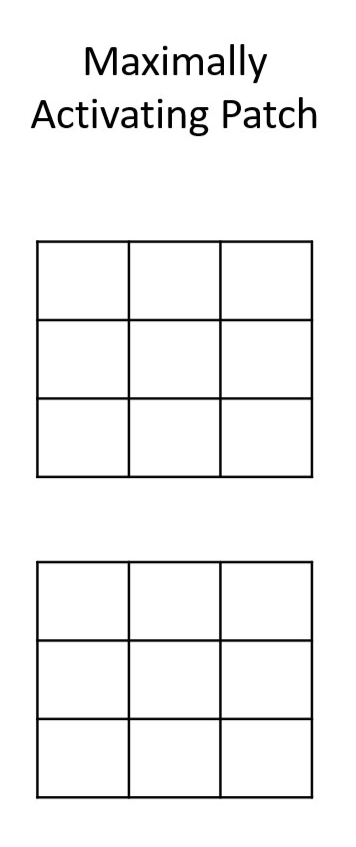
\includegraphics[width=.12\linewidth]{images/conv_question_blanks_2.png}
\end{figure}

\begin{tcolorbox}[title=Solution]
\end{tcolorbox}
